\setlength{\columnsep}{3pt}
\begin{flushleft}
	\bigskip
	\begin{itemize}
		\item A \textbf{hard disk drive (HDD) or hard drive}, is a data storage device that stores and retrieves digital data in computer.
		\item HDD brands in market: Seagate, Western Digital, Hitachi etc.
			\begin{figure}[h!]
				\centering
				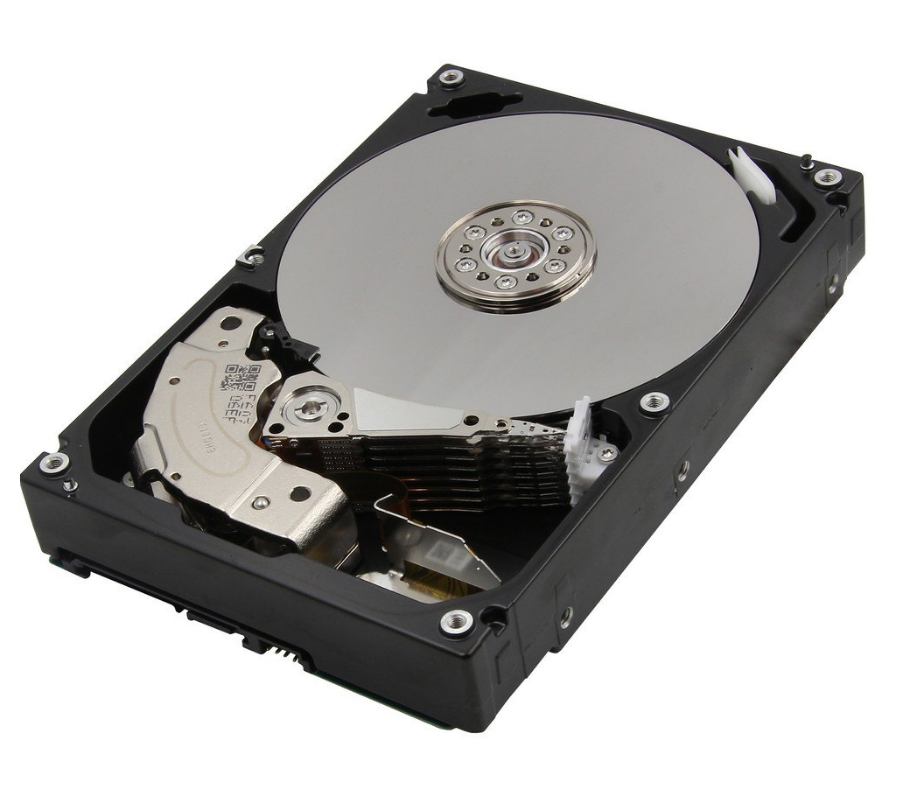
\includegraphics[scale=.3]{content/chapter8/images/hdd.png}
				\caption{Hard disk}
				\label{hard_disk}
			\end{figure}
		\item \textbf{Partitioning} means to divide a HDD into many logical drives.
		\begin{figure}[h!]
			\centering
			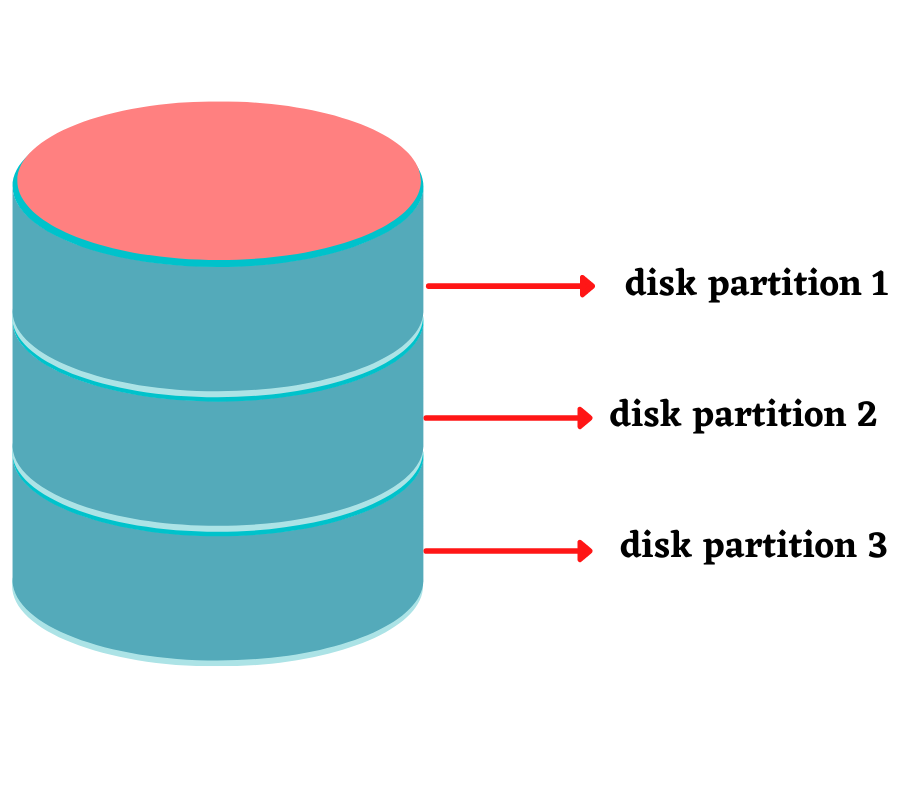
\includegraphics[scale=.3]{content/chapter8/images/part2.png}
			\caption{Hard disk partitions}
			\label{hard_disk_partitions}
		\end{figure}		
	\end{itemize}

\newpage

	
\end{flushleft}

\newpage

